\documentclass[9pt,twocolumn,twoside]{../../styles/osajnl}
\usepackage{fancyvrb}
\journal{i524} 

\title{Apache Spark}

\author[1]{Snehal Chemburkar}
\author[1]{Rahul Raghatate}

\affil[1]{School of Informatics and Computing, Bloomington, IN 47408, U.S.A.}

\affil[*]{Corresponding authors: snehchem@iu.edu, rraghtate@iu.edu}

\dates{project-001, \today}

\ociscodes {Spark, RDDs, DAG, Driver, Cluster, Worker, I524}

% replace this with your url in github/gitlab
\doi{\url{https://github.com/snehalvartak/sp17-i524/paper1/S17-IR-2006/report.pdf}}


\begin{abstract}
Apache Spark, developed at UC Berkeley AMPLAB, is a high performance framework for analyzing large datasets \cite{article-spark-1}. The main idea behind the development of Spark was to create a generalized framework that could process diverse and distributed data as opposed to MapReduce which only support batch processing of data. Spark has multiple libraries built on top of its core computational engine which help process diverse data. This paper will discuss the spark runtime architecture, its core and libraries. \newline
\end{abstract}

\setboolean{displaycopyright}{true}

\begin{document}

\maketitle

\section{Introduction}

Spark is an open source distributed cluster computing engine for
processing the different types of data available these days. The
distribution, scheduling and monitoring of clusters is done by the
Spark core. The high level components required for processing the diverse workloads such as structured or streaming data are powered by the spark core. “These components are designed to inter-operate closely letting
you combine them like libraries in a software project \cite{book-spark}.”

The Spark core and the higher level libraries on top of the core are
tightly integrated meaning when updates or improvements are
implemented in the spark core help improve the spark libraries as
well. Tight integration also makes it easier to write applications
combining different workloads. This is explained nicely in the
following example. One can build an application using machine learning
libraries to process real time data from streaming sources and
analysts can simultaneously access the data using SQL also in real
time.  In this example three different workloads namely SQL, streaming
data and machine learning algorithms can be implemented in a single
system which is a requirement in today’s age of big data.

\section{Spark Components}

Figure \ref{fig:spark-stack} depicts the various building blocks of
the spark stack. The Spark Core is computational engine which performs the task scheduling, distribution, and cluster monitoring tasks. Resilient Distributed Datasets(RDD) \cite{paper-RDD} and Directed Acyclic Graphs(DAG) are two important concepts in Spark. The libraries or packages supporting the diverse workloads are built on top of the Spark core. These packages include Spark SQL, Spark Streaming, MLlib (machine learning library) and GraphX.

\begin{figure}[htbp]
\centering
\fbox{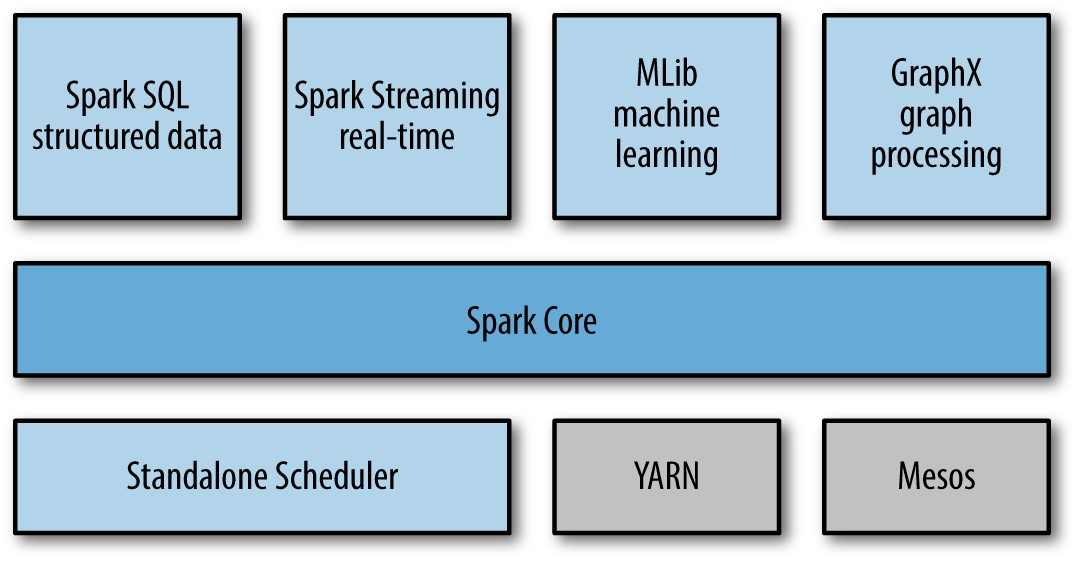
\includegraphics[width=\linewidth]{images/Spark-Components}}
\caption{Spark Components \cite{book-spark}}
\label{fig:spark-stack}
\end{figure}

\subsection{Spark Core}

Spark Core is the foundation framework that provides basic I/O functionality, distributed task scheduling and dispatching.
more \cite{article-spark-1}." 
\subsection{Resilient Distributed Datasets(RDD)}
Resilient Distributed Datasets(RDD) \cite{paper-RDD} are Spark's
primary abstraction, which are a fault-tolerant collection of elements that can be operated in parallel. RDDs are immutable once they are created but they can be transformed or actions can be performed on them \cite{article-spark-1}. Users can create RDDs through external sources or by transforming another RDD. Transformations and Actions are the two
types of operations supported by RDDs.
\begin{enumerate}
\item Transformations: Since RDDs are immutable the transformations return a new RDD and not a single value." Transformations are lazily evaluated, i.e. they are not computed immediately. They are executed
only when an action runs on it. Some of the Transformation functions are map, filter, ReduceByKey, FlatMap and GroupByKey \cite{article-spark-1}."
\item Actions are operations that result in a return
value after computation or triggers a task in response to some
operation.Some Action operations are first, take, reduce,
collect, count, foreach and CountByKey \cite{article-spark-1}.
\end{enumerate}
As such, RDDs are ephemeral disk, which means they do not persist
data, however, users can explicitly persist RDDs to ease data
reuse. Traditional distributed computing systems provide fault
tolerance through checkpoint or data replication. "RDDs provide fault
tolerance by logging the transformations used to build a data set
through (its lineage) rather than actual data \cite{paper-RDD}." If one of the RDD fails, it has enough information about of its lineage so as to recreate the dataset from other RDDs, thus saving cost and time.
\subsection{Directed Acyclic Graph(DAG)}
Directed Acyclic Graph(DAG), which supports a cyclic data flow, "consists of finitely many vertices and edges, with each edge directed from one vertex to another, such that there is no way to start at any vertex v and follow a consistently-directed sequence of edges that eventually loops back to v again \cite{wiki-DAG}." When we run any application in spark, the driver program converts the transformations and actions to logical directed acyclic graphs(DAG). The DAGs are then converted to physical execution plans with a set of stages which are distributed and bundled into tasks. These tasks are distributed among the different worker nodes for execution.

\subsection{Spark SQL}
Spark SQL\cite{book-spark} is a library built on top of the Spark Core to support
querying structured data using SQL or Hive Query Language. It allows
users to perform ETL (Extract, Transform and Load) operations on data
from various sources such as JSON, Hive Tables and Parquet. Developers
can "intermix SQL queries with programmatic data manipulations
supported by RDDs in Python, Java, and Scala, all within a single
application \cite{book-spark}."

\subsection{Spark Streaming}
Spark Streaming \cite{book-spark} library enables Spark to process real time
data. Examples of streaming data are messages being published to a
queue for real time flight status update or the log files for a
production server. "Spark Streaming provides an API for manipulating
data streams that closely matches the Spark Core’s RDD API, making it
easy for programmers to learn the project and move between
applications that manipulate data stored in memory, on disk, or
arriving in real time." Spark Streaming is designed such that it
provides the same level of fault tolerance, throughput and scalability
as the Spark Core.

\subsection{MLlib}
MLlib \cite{book-spark} is rich library of machine learning algorithms for Spark which
can be accessed from Java, Scala as well as Python. It provides Spark
with machine learning algorithms such as “classification, regression,
clustering, and collaborative filtering”. It also provides machine
learning functionality such as “model evaluation and data import”. The
common machine learning algorithms include K-means, navie bayes,
logistic regression, Principal component analysis and so on.

\subsection{GraphX}

GraphX introduces the Resilient Distributed Property
Graph, which is directed multi-graph having properties
attached to each edge and vertex. GraphX includes a set of
operators like aggregateMessages, subgraph and
joinVertices, and optimized variant of Pregel API. It also
includes builders and graph algorithms to simplify graph
analytics tasks \cite{article-spark-1}.

\section{Runtime Architecture}

The runtime architecture of Spark,  illustrated in Figure \ref{fig:spark-runtime}, consists of a driver program, a cluster manager, workers or executors and the HDFS (Hadoop Distributed File System) \cite{article-spark-1}.
Spark uses a master/slave architecture in which the driver program is the master and worker nodes or executors are the slaves. The driver runs the main() method of the user program which creates  the SparkContext, the RDDs and performs transformations and actions \cite{book-spark}.

\begin{figure}[htbp]
\centering
\fbox{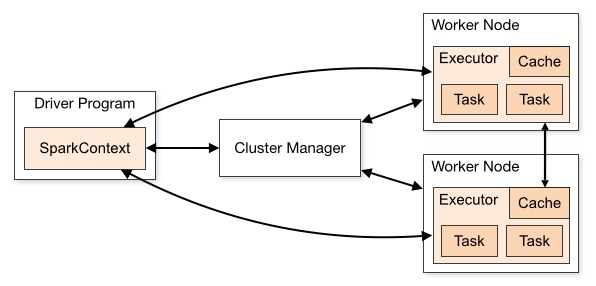
\includegraphics[width=\linewidth]{images/cluster-overview.jpg}}
\caption{Spark Architecture \cite{www-spark-cluster}}
\label{fig:spark-runtime}
\end{figure}

When we launch an application using the Spark Shell it creates a driver program which in turn initializes the SparkContext. Each spark application has its own SparkContext object which is responsible for the entire execution of the job. The SparkContext  object then connects to cluster manager to request resources for its workers. The cluster manager provide executers to worker nodes, which are used to run the logic and also store the application data. The driver will send the tasks to the executors based on the data placement. The executors register themselves with the driver, which helps the driver keep tabs on the executors. Driver can also schedule future tasks by caching or persisting data.
The following Cluster Managers are used in Spark based on the requirement-
\begin{itemize}
    \item Standalone cluster manager is a simple cluster manager built into Spark to manage is own clusters \cite{www-spark-cluster}.
    \item Apache Mesos is a dedicated cluster manager that provides Spark with rich resource scheduling capabilities \cite{www-spark-cluster}.
    \item YARN is the only cluster manager in Spark that provides security support. “It allows dynamic sharing and central configuration of the same pool of cluster resources between various frameworks that run on YARN \cite{www-spark-2}”.
\end{itemize}

\subsection{Educational Resources}
 The Apache Spark website has a detailed documentation on the how to get started with spark \cite{www-apache-spark}. It explains the concepts and shows examples to help us familiarize with Spark.
 
\section*{Acknowledgements}

This paper is written as part of the I524: Big Data and Open Source Software Projects coursework at Indiana University. We would like to thank our Prof. Gregor von Laszewski, Prof. Gregory Fox and the AIs for their help and support

% Bibliography

\bibliography{references}
 
\end{document}
